\chapter{Modellierung}\label{cha:modellierung}

\section{Datenmodellierung}

Modellieren ist der Weg von der realen Welt bis zum Datenmodell. Ein Datenmodell verdeutlicht die Beziehungen zwischen Daten. Ergebnis des Modellierungsprozesses ist ein sogenanntes Datenschema, das zumeist grafisch visualisiert wird.
Im Hinblick auf die Datenmodellierung eignen sich folgende Ansätze:

\paragraph{Konzeptuelles Datenmodell}
Beschreibt die globale logische Struktur aller Daten Implementierungs-unabhängig und stellt diese in einer systematischen Form dar.

\begin{figure}[h]
    \centering
    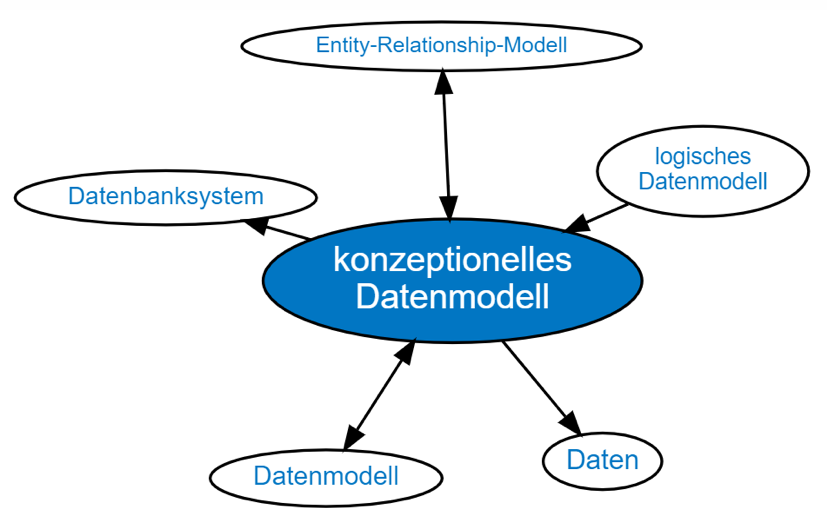
\includegraphics[width=.75\textwidth]{Content/images/modellierung/konzeptionell.png}
    \caption{Konzeptuelles Datenmodell}
    \label{fig:modellierung:konzeptuell}
 \end{figure}

 \paragraph{Logisches Datenmodell}
 Auf die spätere Implementierung ausgerichtetes Datenmodell, das die Daten für den späteren Einsatz bereits vorstrukturiert.

 \begin{figure}[h]
    \centering
    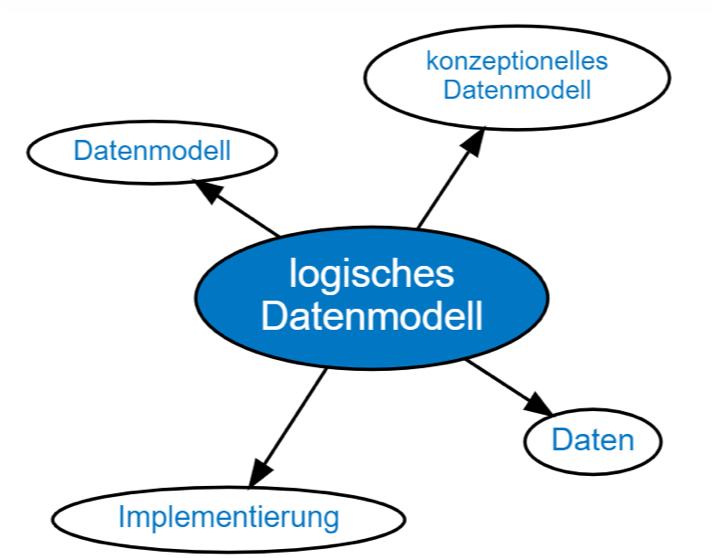
\includegraphics[width=.75\textwidth]{Content/images/modellierung/logisch.png}
    \caption{Logisches Datenmodell}
    \label{fig:modellierung:logisch}
 \end{figure}

 \paragraph{Physisches Datenmodell}
Basiert auf der Grundlage des logischen Datenmodells. Im physischen Datenmodell wird besonders auf Effizienz der SQL-Abfragen geachtet, beispielsweise durch den Entwurf von Indexstrukturen.

Aufgabe der Datenmodellierung ist es, bei der Konzeption eines Informationssystems dessen \emph{Objekte mittels Attribute und Beziehungen gemäß den Anforderungen zu strukturieren} und diese Struktur formal zu dokumentieren.

\emph{Ziele: Redundanzfreie Datenspeicherung und hohe Datenkonsistenz.}
Eine redundanzfreie Datenspeicherung liegt dann vor, wenn jede Information in einer Datenbank genau einmal vorkommt. Des Weiteren muss eine hohe Datenkonsistenz verfolgt werden, so dass Daten eindeutige Informationen darstellen.

\section{Datenmodelle}

Ein Modell ist ein \emph{vereinfachtes Abbild der Wirklichkeit.} Zur Beschreibung der Art und Weise, wie Daten in einer Datenbank gespeichert werden, gibt es verschiedene Datenmodelle. Einige dieser Modelle findet man auch in der betriebswirtschaftlichen Organisationslehre wieder.

\subsection{Hierarchisches Datenmodell}

Das hierarchische Datenmodell kennen wir vom Dateisystem unserer Festplatte (Laufwerksbuchstabe, Ordner, Dateien). Dieses Modell wird auch „Baumstruktur“ genannt. Ganz links (oder oben) befindet sich die Wurzel (Root). Von ihr sind alle Objekte abhängig, die weitere abhängige Objekte haben können. In der betriebswirtschaftlichen Lehre ist es mit einer Stablinienorganisation vergleichbar. Das hierarchische Datenmodell war früher ein sehr gebräuchliches Modell, deshalb bildet es die Grundlage älterer Datenbanksysteme.

\begin{figure}[h]
    \centering
    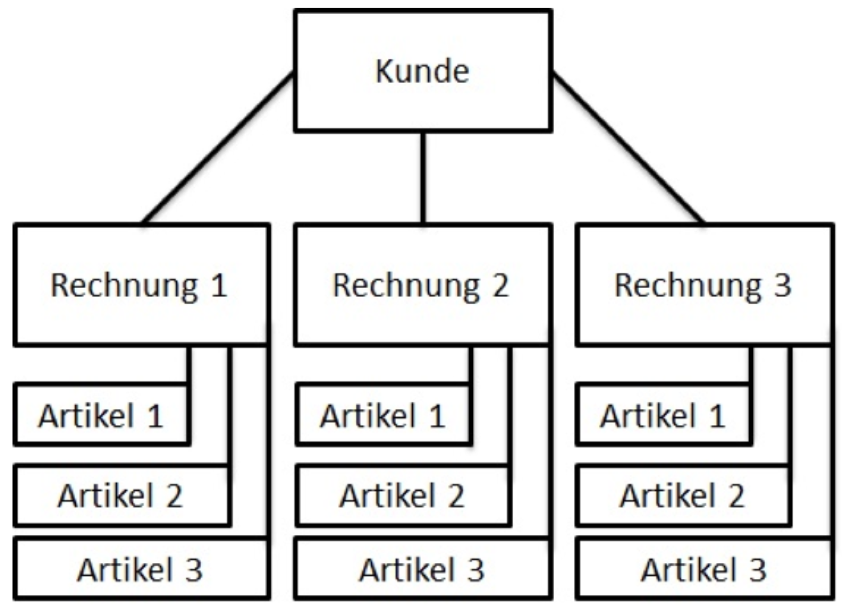
\includegraphics[width=.75\textwidth]{Content/images/modellierung/stablinien.png}
    \caption{Stablinienorganisation}
    \label{fig:modellierung:stablinien}
 \end{figure}

 Durch die \emph{hierarchische Baumstruktur ist der lesende Zugriff extrem schnell.} Der Nachteil der baumstrukturierten Verweise liegt bei der Speicherung der Daten und deren Verknüpfungen, da die Verweise untereinander vorab ermittelt werden müssen. Die Verknüpfungen werden über Eltern-Kind-Beziehungen realisiert und in der Baumstruktur abgebildet. Der große Nachteil bei diesem Modell ist es, dass man nur eine Baumstruktur verwenden kann: Es ist also nicht möglich, zwei Baumstrukturen miteinander zu verknüpfen. \emph{Das hat zur Folge, dass dieses Modell sehr starr ist und wenig Freiheit für den Entwickler bietet. }

 \subsection{Netzwerk Datenmodell}

Definition: Datenmodell, mit dem Netzwerkstrukturen zwischen Datensätzen beschrieben werden können.
Es dient als Grundlage vieler Datenbanksysteme. Die drei Datenbanksprachen DML, DDL und DCL werden angewandt. Durch das netzwerkartige Modell existieren meist unterschiedliche Suchwege, um einen bestimmten Datensatz zu ermitteln. Es ähnelt dem hierarchischen Datenbankmodell und kann einer Matrixorganisation gegenübergestellt werden. 
Das Netzwerk Datenbankmodell besitzt keine strenge Hierarchie. Ein Datenfeld besteht aus einem Namen und einem Wert.
Es sind m:n Beziehungen möglich, d.h. ein Datensatz kann mehrere Vorgänger haben. Des Weiteren können auch mehrere Datensätze an erster Stelle stehen. Der Vorteil dieses Modells ist, das es unterschiedliche Suchwege als Lösungsweg angibt, was natürlich auch zu Problemen führen kann, wenn der Entwickler genau einen Lösungsweg benutzen will. Auch die Übersichtlichkeit verringert sich, wenn das Modell ständig weiter wächst.

\begin{figure}[h]
    \centering
    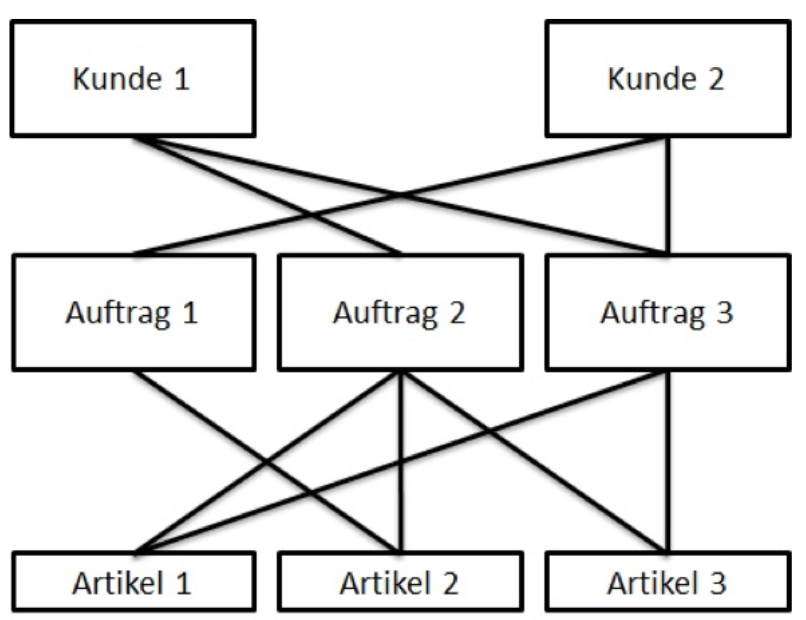
\includegraphics[width=.75\textwidth]{Content/images/modellierung/netzwerk.png}
    \caption{Netzwerk Datenmodell}
    \label{fig:modellierung:netzwerk}
 \end{figure}

 Heute wird das Netzwerkdatenbankmodell als eine Art Verallgemeinerung des hierarchischen Datenbankmodells gesehen.

 \subsection{Relationales Datenmodell}

 = Auf den Arbeiten von Edgar F. Codd von 1970 basierendes Datenmodell, mit dem Beziehungen zwischen Daten in Form von Relationen beschrieben werden. 

In einfachen Worten: Ein relationales Datenmodell ist eine Ansammlung von Tabellen, die miteinander verknüpft sind.
Das relationale Datenmodell ist das am weitesten verbreitete Datenmodell, welches in der Datenbankentwicklung als Standard genutzt wird. Das Fundament des Datenbankmodells besteht aus drei Elementen: Tabellen, Attributen und Beziehungen.

\paragraph{Vorteile:} sehr einfach und flexibel zu erstellen, hohe Flexibilität, leichte Handhabung
\paragraph{Nachteil:} Effizienzprobleme bei großem Datenvolumen

Die wichtigsten Operationen mit Relationen (relationale Algebra), die ein Datenbankmanagementsystem zur Verfügung stellen muss, sind folgende:

\begin{itemize}
    \item Auswahl von Zeilen
    \item Auswahl von Spalten
    \item Aneinanderfügen von Tabellen
    \item Verbund von Tabellen
\end{itemize}

\subsubsection{Entität}

Als Entität wird in der Datenmodellierung ein eindeutig zu bestimmendes Objekt bezeichnet, über das Informationen gespeichert oder verarbeitet werden sollen. Ein Entitätstyp beschreibt die Ausprägungen eines Objektes durch die Angabe von Attributen. Durch Typisierung (Erkennen gleicher Attribute von Entitäten) können Entitätstypen abgeleitet werden – aus mehreren Personen werden z.B. Kunden. Eine Entität kann materiell oder immateriell, konkret oder abstrakt sein. Beispiele für Entitäten: Fahrzeug, Konto, Person.

\subsubsection{Attribute in einer Entität}

Jede Entität besitzt eine bestimmbare Anzahl an Attributen (Ausprägungen bzw. Eigenschaften), die sich eindeutig von anderen Entitäten des gleichen Entitätstyps abgrenzen. Eine Eigenschaft ist ein konkreter Attributwert, den ein zuvor definiertes Attribut annehmen kann. Die Attribute stellen einen „Bauplan“ dar, der eine abstrakte Abbildung der Wirklichkeit ist.

\begin{figure}[h]
    \centering
    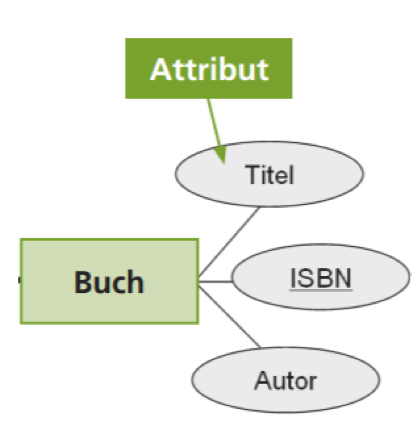
\includegraphics[width=.4\textwidth]{Content/images/modellierung/entity.png}
    \caption{Attribute einer Entity}
    \label{fig:modellierung:entity}
 \end{figure}

 Die Attribute in einer Entität können unterschiedlich aufgebaut sein. Man unterscheidet zwischen \emph{zusammengesetzte, mehrwertige und abgeleitete} Attribute.

 \paragraph{Zusammengesetzte Attribute} bestehen aus der Kombination mehrerer Attribute, die inhaltlich zusammengehören. Anhand einer Firmenadresse wird dies deutlich. Die Firmenadresse selbst ist ein Attribut der Firma, sie enthält aber die Attribute Straße, Hausnummer, Postleitzahl und Ort.

 \paragraph{Mehrwertige Attribute} können einen oder mehrere Attributwerte aufnehmen. So könnte ein Student gleichzeitig in zwei Studiengänge eingeschrieben sein.

 \paragraph{Abgeleitete Attribute} werden aus anderen Attributen oder Entitäten berechnet. Bezogen auf eine Datenbank wäre das z.B. die Bildung einer Summe aus mehreren Spalten einer Tabelle.

 \subsection{Beziehungen in Datenbanken}

 Zwischen Relationen (Tabellen/Entitäten) können Beziehungen in einer Datenbank bestehen. Angenommen man hat eine Relation „Mutter“ und eine Relation „Kind“ – denkbar wären nun vier Möglichkeiten von Assoziationen/Beziehungen zwischen den Tabellen.

 In einem Datenbankmodell können folgende Beziehungen auftreten:

 \begin{itemize}
     \item Jede Mutter hat exakt ein Kind (1)
     \item Jede Mutter hat ein oder kein Kind (c)
     \item Jede Mutter hat mindestens ein Kind (m)
     \item Jede Mutter hat eine kein, ein, oder eine beliebige Anzahl von Kindern (mc)
 \end{itemize}

 \subsection{Kardinalität}

 Die Kardinalität zwischen dem Entitätstyp 1 und dem Entitätstyp 2 gibt an, wie viele Entitäten des Entitätstyps 2 höchstens mit einer Entität des Entitätstyps 1 in Beziehung stehen. Die Kardinalität von Beziehungen ist in relationalen Datenbanken in folgenden Formen vorhanden: 
 1:1 Beziehung, 1:n Beziehung und m:n Beziehung. Des Weiteren gibt es noch die sogenannte \emph{Modifizierte Chen-Notation} (c).
 
 \subsubsection{1:1 Beziehung}

 In einer „eins zu eins“ Beziehung in relationalen Datenbanken ist jeder Datensatz in Tabelle A genau einem Datensatz in Tabelle B zugeordnet und umgekehrt. Diese Art von Beziehung sollte in der Modellierung vermieden werden, weil die meisten Informationen, die auf diese Weise in Beziehung stehen, sich in einer Tabelle befinden können. Eine 1:1 Beziehung verwendet man nur, um eine Tabelle aufgrund ihrer Komplexität zu teilen oder um einen Teil der Tabelle aus Gründen der Zugriffsrechte zu isolieren.

 \begin{figure}[h]
    \centering
    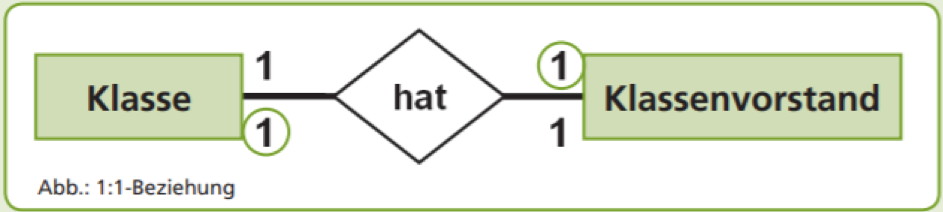
\includegraphics[width=.8\textwidth]{Content/images/modellierung/11.png}
    \caption{Eine Klasse hat einen Klassenvorstand. Ein Klassenvorstand hat eine Klasse}
    \label{fig:modellierung:11}
 \end{figure}

 \subsubsection{1:n Beziehung}

 Eine „eins zu viele“ Beziehung in relationalen Datenbanken ist der häufigste Beziehungstyp in einer Datenbank. In einer 1:n Beziehung können einem Datensatz in Tabelle A mehrere passende Datensätze in Tabelle B zugeordnet sein, aber einem Datensatz in Tabelle B ist nie mehr als ein Datensatz in Tabelle A zugeordnet. Eine 1:n Beziehung wird mit einem Fremdschlüssel aufgelöst.
Als Fremdschlüssel in der abhängigen Relation (n-Seite) wird der Primärschlüssel der unabhängigen Relation (1-Seite) eingefügt. Er verweist daher auf eine Zeile in dieser Relation.

\begin{figure}[h]
    \centering
    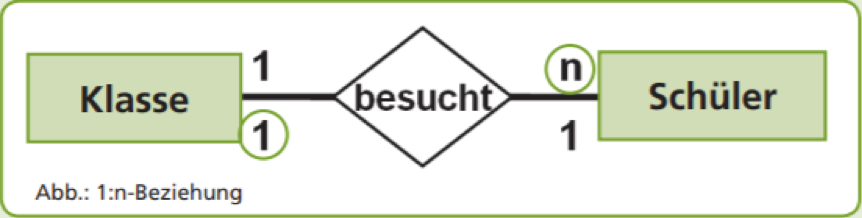
\includegraphics[width=.8\textwidth]{Content/images/modellierung/1n.png}
    \caption{Eine Klasse hat mehrere Schüler. Ein Schüler besucht 1 Klasse}
    \label{fig:modellierung:1n}
 \end{figure}

 \subsubsection{m:n Beziehung}

 Bei „viele zu viele“ Beziehung in relationalen Datenbanken können jedem Datensatz in Tabelle A mehrere passende Datensätze in Tabelle B zugeordnet sein und umgekehrt. Diese Beziehungen können nur über eine dritte Tabelle, eine Verbindungstabelle C, realisiert werden. Die Verbindungstabelle C enthält die beiden Primärschlüssel der Tabellen A und B als Fremdschlüssel. Der Primärschlüssel der Verbindungstabelle wird aus diesen beiden Fremdschlüsseln gebildet. Daraus folgt, dass eine m:n Beziehung in Wirklichkeit zwei 1:n Beziehungen sind.

\begin{figure}[h]
    \centering
    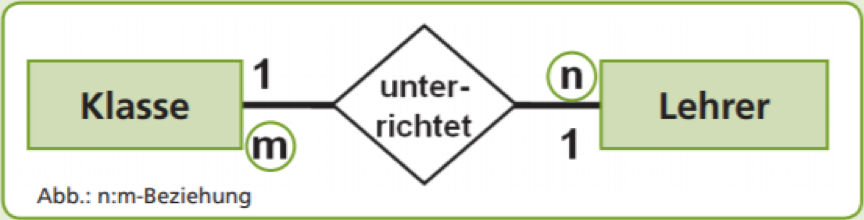
\includegraphics[width=.8\textwidth]{Content/images/modellierung/mn.png}
    \caption{Eine Klasse wird von mehreren Lehrern unterrichtet. Ein Lehrer unterrichtet mehrere Klassen.}
    \label{fig:modellierung:mn}
\end{figure}

\begin{figure}[h]
    \centering
    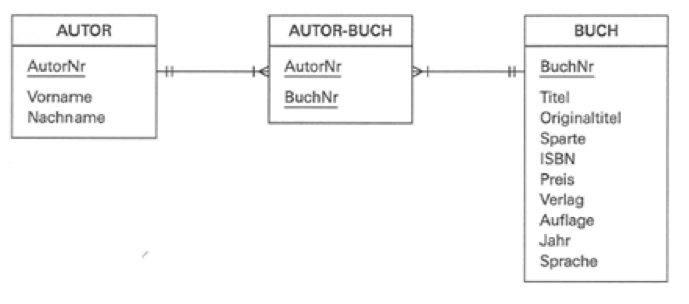
\includegraphics[width=.8\textwidth]{Content/images/modellierung/autorbuch.png}
    \caption{Verbindungstabelle zwischen Autor und Buch}
    \label{fig:modellierung:mn}
\end{figure}

\subsubsection{Conditional c}

Die obigen 3 Beziehungen sind die Standardbeziehungen. Diese wird Chen Notation genannt. Bei der modifizierten Chen Notation gibt es zusätzlich noch das conditional c. Dieser Buchstabe repräsentiert „eine oder keine“ (1:c) Beziehungen und wird beispielsweise bei der Generalisierung angewandt (siehe Kapitel Generalisierung/Spezialisierung). Daraus ergeben sich nun folgende zusätzliche Beziehungen:

\begin{itemize}
    \item 1:c Beziehung: Schüler (1) besitzt Buchausweis (c)
    \item 1:mc Beziehung: Schüler (1) startet Druckaufträge (mc)
    \item c:c Beziehung: Schüler (c) mietet Spind (c)
    \item c:m Beziehung: Religionslehrer (c) unterrichtet Schüler (m)
    \item c:mc Beziehung: Schüler (c) recherchiert im Lexikon (mc)
    \item m:mc Beziehung: Schüler (m) hat Robotik Unterricht (mc)
    \item mc:mc Beziehung: Schüler (mc) benutzt Onlinelexika (mc)
\end{itemize}

Jede Zeile (auch Tupel genannt) in einer Tabelle ist ein Datensatz. Jedes Tupel besteht aus einer großen Reihe von Eigenschaften (Attributen), den Spalten der Tabelle. Ein Relationsschema legt dabei die Anzahl und den Typ der Attribute für eine Tabelle fest.

Das relationale Datenmodell erhält man, indem man das hierarchische Datenmodell mit dem Netzwerk-Datenmodell kombiniert. Ein Datenobjekt ist von einem oder mehreren Datenobjekten abhängig. Daraus ergeben sich mehrere Arten von Abhängigkeiten, die wir als Beziehungen bezeichnen.

\begin{figure}[h]
    \centering
    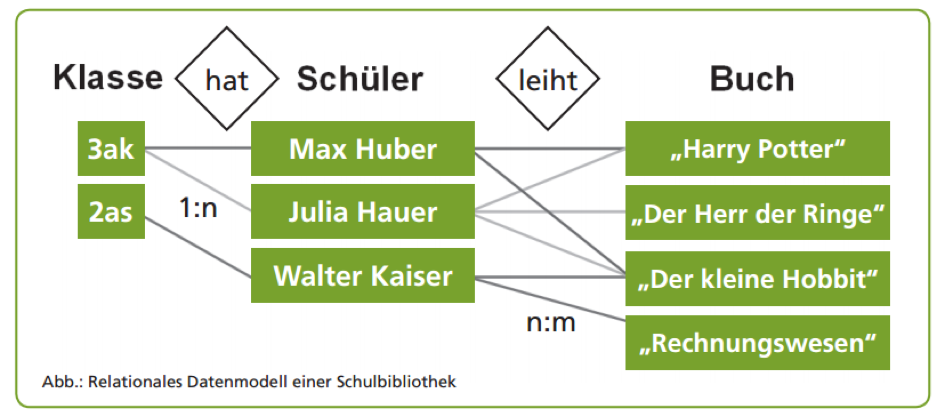
\includegraphics[width=.8\textwidth]{Content/images/modellierung/biblio.png}
    \caption{}
    \label{fig:modellierung:biblio}
\end{figure}

Des Weiteren können Verknüpfungen (Beziehungen) über sogenannte Primärschlüssel hergestellt werden, um bestimme Attribute, die den gleichen Primärschlüssel oder in einer Detailtabelle als Fremdschlüssel besitzen, abzufragen.

\subsubsection{Primary Keys}

Der Primärschlüssel kommt in relationalen Datenbanken zum Einsatz und wird zur eindeutigen Identifizierung eines Datensatzes verwendet. Neben der Eindeutigkeit soll ein Primärschlüssel kurz sein und leicht geschrieben werden können. Des Weiteren sollen aus dem Schlüssel gewisse Eigenschaften der Entität ersichtlich sein. Diese Eigenschaft kann im Widerspruch zu der Eindeutigkeit und der Kürze stehen. 
Beispiele:
\begin{itemize}
    \item Sozialversicherungsnummer (nnnn dd mm yy) besteht aus einer 4-stelligen Nummer und den Geburtsdaten - Eindeutigkeit: ja, Kürze: teilweise, Sprechender Schlüssel: kaum
    \item Matrikelnummer eines Studenten (yysssnnn) besteht aus dem Immatrikulationsjahr, einer Studienkennzahl und einer laufenden Nummer - Eindeutigkeit: ja, Kürze: ja, Sprechender Schlüssel: teilweise
\end{itemize}

In einer normalisierten Datenbank besitzen alle Tabellen einen Primärschlüssel.
Der Wert eines Primärschlüssels muss in einer Tabelle einmalig sein, da er jeden Datensatz eindeutig kennzeichnet. Des Weiteren wird er häufig als Datenbank-Index verwendet, um die Daten auf der Festplatte abzulegen. Der Primärschlüssel einer Relation kann unterschiedlich aufgebaut sein. Man unterscheidet zwischen eindeutigen, zusammengesetzten und künstlichen Primärschlüsseln.

\paragraph{Eindeutiger Primary Key}
Hierbei handelt es sich um einen eindeutigen Schlüssel, der in einer Spalte der Tabelle gespeichert wird. Als Spalte kann ein Attribut des Datensatzes verwendet werden, das für jeden Eintrag in der Tabelle einen einmaligen Wert annimmt. Als eindeutiges Primärschlüssel-Attribut könnte beispielsweise die Sozialversicherungsnummer in einer Mitarbeitertabelle verwendet werden.

\paragraph{Zusammengesetzter Primary Key}
Ist ein Datensatz anhand eines Attributes nicht eindeutig identifizierbar, so kann der Primärschlüssel auch aus einer Kombination mehrerer Attribute bestehen. Dabei muss sichergestellt werden, dass jede dieser Kombinationen nur einmalig auftritt. Ein zusammengesetzter Primärschlüssel kann z.B. der Vor- und Nachname in Kombination mit dem Geburtsdatum sein.

\paragraph{Künstlicher Primary Key}
Gibt es in einer Tabelle keine eindeutigen Spalten bzw. Kombinationen aus Spalten, so kann auch auf einen künstlichen Schlüssel zurückgegriffen werden. Dieser ist auch als Surrogate Key bekannt und wird als zusätzliche Spalte in einer Tabelle eingefügt. In der Praxis wird häufig eine fortlaufende Ganzzahlen-Folge verwendet, um einen Datensatz eindeutig identifizieren zu können.

\subsubsection{Foreign Key}

Der Fremdschlüssel kann Bestandteil einer Tabelle in einer relationalen Datenbank sein. Dabei handelt es sich um eine Schlüsselspalte, die auf einen Primärschlüssel einer anderen oder aber derselben Tabelle verweist. In einfachen Worten: Als Fremdschlüssel wird eine Menge von Attributen bezeichnet, die in einer anderen Tabelle den Primärschlüssel bildet. 1:n Beziehungen werden beispielsweise mit einem Fremdschlüssel aufgelöst. 

\begin{figure}[h]
    \centering
    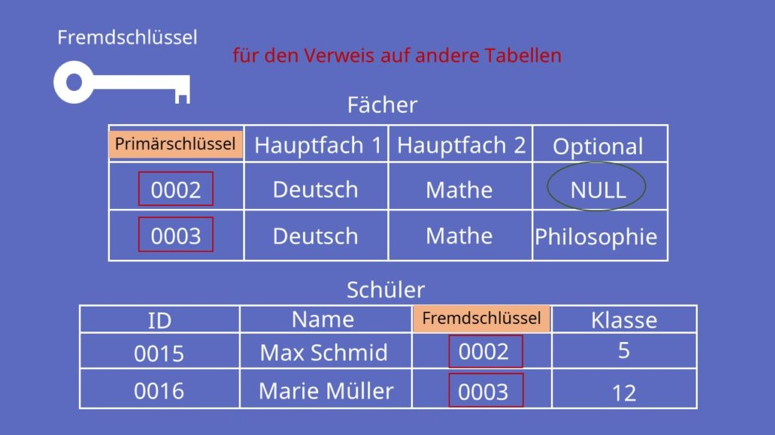
\includegraphics[width=.8\textwidth]{Content/images/modellierung/foreignkey.png}
    \caption{Foreign Key}
    \label{fig:modellierung:foreignkey}
\end{figure}

\subsection{Objekt-Datenmodell}

Objekte sind modellhafte Abbilder der Wirklichkeit. Das Objekt-Datenmodell wird vor allem im Bereich der Softwareentwicklung eingesetzt. Ein wichtiges Prinzip beim Objektmodell ist die Vererbung, durch die ein effizienteres Programmieren möglich wird.

\begin{figure}[h]
    \centering
    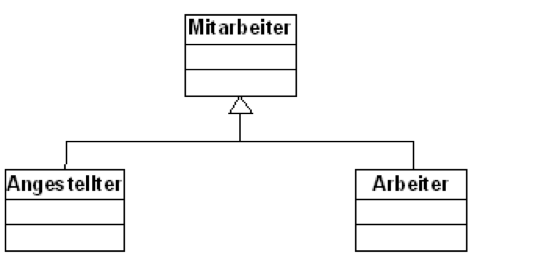
\includegraphics[width=.8\textwidth]{Content/images/modellierung/objekt.png}
    \caption{Vererbung bei Objekten}
    \label{fig:modellierung:objekt}
\end{figure}

\section{Entity-Relationship-Modell}

Die Modellierung relationaler Datenbanken erfolgt mit dem von Peter Chen entwickelten Entity-Relationship-Modell. Bevor mittels SQL angefangen wird, Tabellen und Beziehungen anzulegen, wird zuerst geplant, wie die Datenbankstruktur funktionieren und aufgebaut werden soll. Der Einsatz von ER-Modellen ist in der Praxis ein gängiger Standard für die Datenmodellierung, auch wenn es unterschiedliche grafische Darstellungsformen von Datenbankmodellen gibt.
Mithilfe des Entity-Relationship-Modells soll eine Typisierung von Objekten, ihrer relationalen Beziehungen untereinander und der zu überführenden Attribute, stattfinden.

\paragraph{Bestandteile des ERD}
\begin{itemize}
    \item \textbf{Entität:} Ein individuell identifizierbares Objekt der Wirklichkeit.
    \item \textbf{Beziehung}: Eine Verknüpfung / Zusammenhang zwischen zwei oder mehreren Entitäten.
    \item \textbf{Attribut:} Eine Eigenschaft, die im Kontext zu einer Entität steht.
\end{itemize}

\begin{figure}[h]
    \centering
    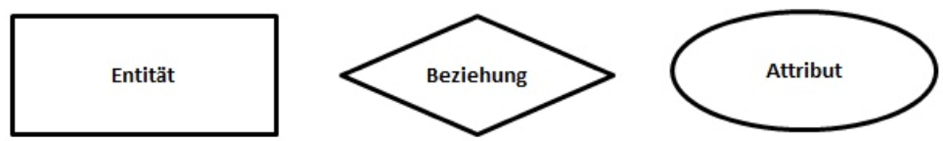
\includegraphics[width=.8\textwidth]{Content/images/modellierung/erd.png}
    \caption{UML Darstellung}
    \label{fig:modellierung:erd}
\end{figure}
\begin{figure}[h]
    \centering
    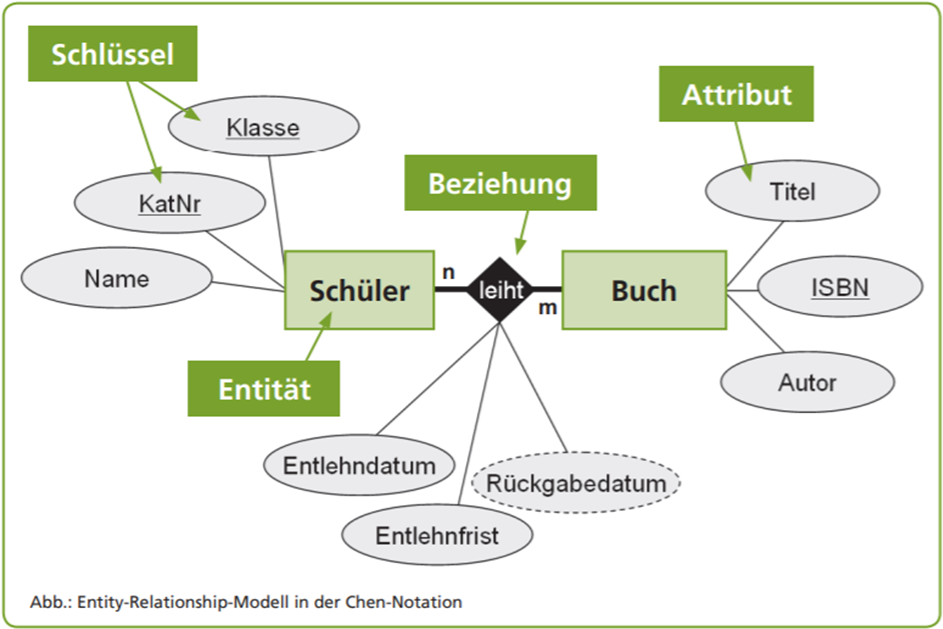
\includegraphics[width=.8\textwidth]{Content/images/modellierung/erde.png}
    \caption{Was ist was}
    \label{fig:modellierung:erde}
\end{figure}

\textit{Beispiel}

\begin{figure}[h]
    \centering
    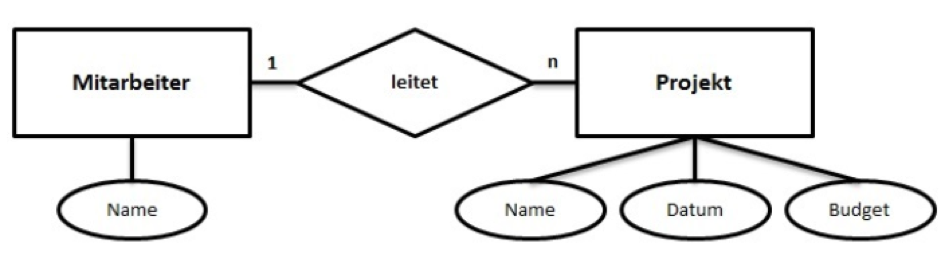
\includegraphics[width=.8\textwidth]{Content/images/modellierung/bsp.png}
    \caption{Beispiel Darstellung}
    \label{fig:modellierung:bsp}
\end{figure}
\textit{Erklärung:}
Ein Mitarbeiter hat einen Namen. Ein Projekt hat einen Namen, ein Datum und ein Budget. Ein Mitarbeiter kann mehrere Projekte leiten, aber ein Projekt kann nur von einem Mitarbeiter geleitet werden. 
Zur Wiederholung: Diese Notation nennt man Chen-Notation und ist ein gängiger Standard in der Praxis der Datenmodellierung.

\subsection{Überleitung eines ERD’s in ein relationales Modell}

Ausgangspunkt ist ein vollständiges ER-Diagramm. Ziel ist die Darstellung des Sachverhaltes in Form von Relationen (Tabellen). Eine Tabelle ist eine Menge von Tupeln; ein Tupel ist eine Liste von Werten und entspricht einer Tabellenzeile.

\begin{figure}[h]
    \centering
    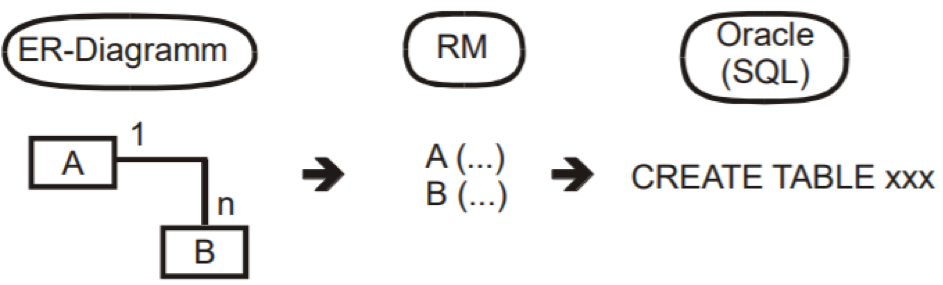
\includegraphics[width=.8\textwidth]{Content/images/modellierung/erdtor.png}
    \caption{ERD zu Relational}
    \label{fig:modellierung:erdtor}
\end{figure}

\begin{center}
    \begin{tabular}{ | l | p{0.6\textwidth} |}
        \hline
        \multicolumn{2}{|c|}{\textbf{Merkmale einer Tabelle}} \\ \hline
        Name & eine Tabelle hat einen eindeutigen Namen
        z.B. ARTIKEL \\ \hline
        Zeilen & sie hat mehrere Tupel (Tabellenzeilen). Die Ordnung der Tupel ist bedeutungslos, weil eine Zeile nicht aufgrund ihrer Position, sondern aufgrund von Werten angesprochen wird.
        z.B.: (300, Müller, 4060, Leonding)        \\ \hline
        Spalten & sie hat mehrere Spalten (Eigenschaften). Die Ordnung der Spalten ist bedeutungslos, weil eine Eigenschaft nicht aufgrund der Position, sondern aufgrund ihres Namens angesprochen wird; dieser Name ist eindeutig
        z.B. Ort   \\ \hline     
        Werte & Eine bestimmte Spalte enthält Attributwerte als Daten
        z.B. Leonding\\ \hline        
    \end{tabular}
\end{center}

\begin{center}
    \begin{tabular}{ | p{0.3\textwidth} | p{0.7\textwidth} | }
        \hline
        1. Jede Entitätsmenge wird als Tabelle mit einem Primärschlüssel dargestellt & Strukturregel 1 (SR1): Bei der Darstellung von Entitätsmengen durch Relationen muss für jede Relation ein Primärschlüssel existieren \\ \hline     
        2. 1:n Beziehungen werden Fremdschlüssel & Als Fremdschlüssel in der abhängigen Relation (n-Seite) wird der Primärschlüssel der unabhängigen Relation (1-Seite) eingefügt. 
        Er verweist daher auf eine Zeile in dieser Relation.
        (ähnlich einem Pointer oder einem Link) \\ \hline
        3. m:n Beziehungen werden assoziative Tabellen & Die neu gebildete assoziative Relation enthält die Primärschlüssel der beiden in Beziehung stehenden Relationen. Sie erhält ihren Primärschlüssel entweder direkt als Kombination der beiden Fremdschlüssel oder es wird („künstlich“) ein neuer Primärschlüssel zugeteilt; die beiden Fremdschlüssel werden dann als Nichtschlüsselattribute verwendet. \\ \hline
        4. Eigenschaften werden Spalten & Alle Eigenschaften werden als Attribute abgebildet. Die Eigenschaftswerte finden sich dann in der Spalte „darunter“. \\ \hline
        5. Jede Beziehung wird zu einem Fremdschlüssel & Auch 1:1 – Beziehungen und insbesondere rekursive Beziehungen werden als Fremdschlüssel abgebildet. \\ \hline
        6. Normalisierung & Prof. Kainerstorfer um Skript bitten (1.4) \\ \hline
        7. Aggregation & Prof. Kainerstorfer um Skript bitten (1.4) \\ \hline
    \end{tabular}
\end{center}

\subsection{Kochrezept - Auflösung m:n Beziehungen}

Im ERD können m:n - Beziehungen vorkommen, diese müssen jedoch spätestens bei der Überleitung in das Relationale Modell aufgelöst werden. Grund: Die Abbildung durch eine Menge von Fremdschlüsseln widerspricht der Forderung nach skalaren Attributen.
Diese Auflösung erfolgt durch die Einführung einer neuen, sogenannten assoziativen Tabelle, die die Fremdschlüssel der beiden in Beziehung stehenden Entitäten enthält. (siehe \ref{fig:modellierung:mitproj})

\begin{figure}[h]
    \centering
    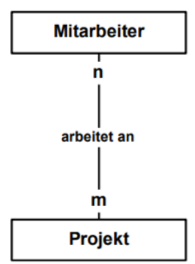
\includegraphics[width=.3\textwidth]{Content/images/modellierung/mitarbeiterprojekt.png}
    \caption{Beispiel}
    \label{fig:modellierung:mitproj}
\end{figure}

Würde man nach der Methode der Überleitung für 1:n - Beziehungen vorgehen, so würde man eine der beiden Lösungen erhalten: (siehe \ref{fig:modellierung:mitproj2})

\begin{figure}[h]
    \centering
    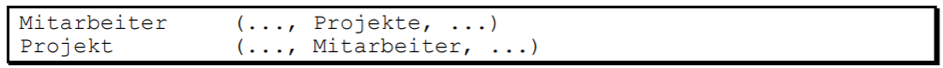
\includegraphics[width=.8\textwidth]{Content/images/modellierung/mitproj.png}
    \caption{Beispiel}
    \label{fig:modellierung:mitproj2}
\end{figure}

Das neue „Attribut“ Mitarbeiter.Projekte müsste alle jene ProjektId’s aufnehmen, an denen der Mitarbeiter arbeitet – und umgekehrt für Projekt.Mitarbeiter. Weil das aber jeweils ganze Mengen sind, und solche Konstrukte in Relationalen Modell nicht definiert sind, führt man eine sogenannte assoziative Relation ein – also eine Relation, die eine Assoziation darstellt. (siehe \ref{fig:modellierung:mitproj3})

\begin{figure}[h]
    \centering
    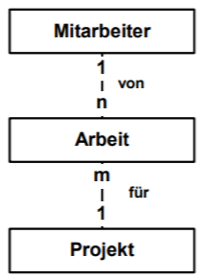
\includegraphics[width=.3\textwidth]{Content/images/modellierung/mitproj3.png}
    \caption{Beispiel}
    \label{fig:modellierung:mitproj3}
\end{figure}

Die Relation Arbeit enthält dann die Fremdschlüssel von Mitarbeiter und Projekt – diese können auch gleichzeitig die Primärschlüssel der neu gebildeten Relation sein (muss aber nicht): (siehe \ref{fig:modellierung:mitproj4})

\begin{figure}[h]
    \centering
    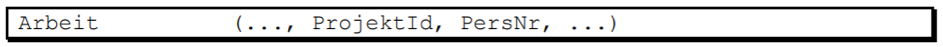
\includegraphics[width=.8\textwidth]{Content/images/modellierung/mitproj4.png}
    \caption{Beispiel}
    \label{fig:modellierung:mitproj4}
\end{figure}

\section{Aggregation}

Eine Aggregatfunktion ist eine Funktion, die gewisse Eigenschaften von Daten zusammenfasst.
Man unterscheidet:

\begin{itemize}
    \item Distributive Funktionen
    \begin{itemize}
        \item Summe (SUM)
        \item Anzahl (COUNT)
        \item Maximum (MAX)
        \item Minimum (MIN)
    \end{itemize}
    \item Algebraische Funktionen
    \begin{itemize}
        \item Mittelwert (AVG)
    \end{itemize}
    \item weitere Funktionen
    \begin{itemize}
        \item Standardabweichung (StDev)
        \item Standardabweichung für die Grundgesamtheit (StDevP)
        \item Median
    \end{itemize}
\end{itemize}

\subsection{„is-part-of“-Beziehung (ERM)}

Eine andere Verwendung des Begriffs Aggregation ist auch beim Entity-Relationship-Modell zu finden. So können hier mehrere Einzelobjekte logisch zu einem Gesamtobjekt zusammengefasst werden. Dies geschieht mit der „is-part-of“-Beziehung.

Werden mehrere Einzelobjekte (z.B. Person und Hotel) zu einem eigenständigen Einzelobjekt (z.B. Reservierung) zusammengefasst, dann spricht man von Aggregation. Dabei wird das übergeordnet eigenständige Ganze Aggregat genannt. Die Teile, aus denen es sich zusammensetzt, heißen Komponenten. Aggregat und Komponenten werden als Entitätstyp deklariert.

Bei einer Aggregation wird zwischen Rollen- und Mengenaggregation unterschieden:
Eine Rollenaggregation liegt vor, wenn es mehrere rollenspezifische Komponenten gibt und diese zu einem Aggregat zusammengefasst werden.

Beispiel: 
Fußballmannschaft is-part-of Fußballspiel und Spielort is-part-of Fußballspiel
 	und in anderer Leserichtung:
Fußballspiel besteht-aus Fußballmannschaft und Spielort.
Eine Mengenaggregation liegt vor, wenn das Aggregat durch Zusammenfassung von Einzelobjekten aus genau einer Komponente entsteht.

Beispiel:
\textit{Fußballspieler is-part-of Fußballmannschaft} \newline
 	und in anderer Leserichtung: \newline
\textit{Fußballmannschaft besteht-aus (mehreren, N) Fußballspielern.}

\textit{Generalisierung / Spezialisierung}

Zur weiteren Strukturierung der Entitätstypen wird die Generalisierung eingesetzt. Hierbei werden Eigenschaften von ähnlichen Entitätstypen einem gemeinsamen Obertyp, auch „Superentität“ genannt, zugeordnet. 

Bei diesem Modellierungs-Konstrukt werden gemeinsame Eigenschaften von Entitäten nur einmal modelliert.

\begin{itemize}
    \item Der Generalisierungstyp enthält die Attribute, die alle Entitäten gemeinsam haben.
    \item Die Spezialisierungstypen enthalten die speziell für sie zutreffenden Attribute, wobei
    \begin{itemize}
        \item die Spezialisierung disjunkt (=getrennt) oder überlappend sein kann
        \item die Eigenschaften der Generalisierung erbt
    \end{itemize}
\end{itemize}

\begin{figure}[h]
    \centering
    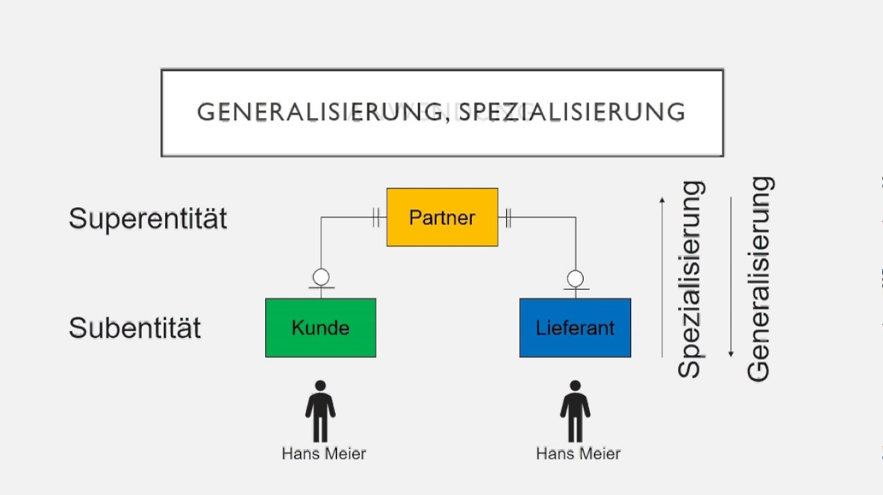
\includegraphics[width=.8\textwidth]{Content/images/modellierung/general.png}
    \caption{Generalisierung und Spezialisierung}
    \label{fig:modellierung:general}
\end{figure}

Diese Beziehungstypen werden durch „is-a“ | „can-be“ beschrieben.

Beispiel:
\textit{Flugreise is-a Reise} \newline
 	und in anderer Leserichtung: \newline
\textit{Reise can-be Flugreise}

Während Spezialisierungen durch Bildung von Teil-Entitätsmengen aus gegebenen Entitäten entstehen, werden bei der Generalisierung gemeinsame Eigenschaften und Beziehungen, die in verschiedenen Entitätstypen vorkommen, zu einem neuen Entitätstyp zusammengefasst. So können z.B. Kunden und Lieferanten zusätzlich zu Geschäftspartnern zusammengeführt werden, da Name, Anschrift, Bankverbindung etc. sowohl bei den Kunden als auch bei den Lieferanten vorkommen.

\section{Unterschied Aggregation und Generalisierung/Spezialisierung}

Generalisierung: bottom-up. \newline
Spezialisierung: top-down.

Bei einer Aggregation werden die Beziehungen zwischen 2 Entitäten (von außen) als eine einzige Entität gesehen, es können jedoch beide Entitäten eigenständig ohne der anderen existieren. 
Beispiel: 

\begin{figure}[h]
    \centering
    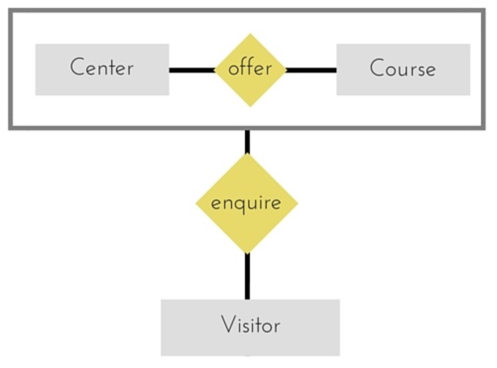
\includegraphics[width=.8\textwidth]{Content/images/modellierung/spez.png}
    \caption{Generalisierung und Spezialisierung}
    \label{fig:modellierung:special}
\end{figure}

Bei einer Aggregation gibt es KEINE VERERBUNG, bei der Generalisierung/Spezialisierung schon.

\section{Data Dictionary}

Ein Data-Dictionary – deutsch Datenwörterbuch, Datenkatalog – ist ein Katalog von Metadaten, der die Definitionen und Darstellungsregeln für alle Anwendungsdaten eines Unternehmens und die Beziehungen zwischen den verschiedenen Datenobjekten enthält, damit der Datenbestand redundanzfrei und einheitlich strukturiert wird. 

Bei einer relationalen Datenbank ist ein Datenwörterbuch eine Menge von Tabellen und Views, die bei Abfragen nur gelesen werden (read-only). Datenbankobjekte, die dort nicht eingetragen sind, gibt es auch nicht. Die Informationen in einem Data Dictionary beinhalten die Namen der Tabellen und deren Spalten inklusive Datentypen und Längen. Es werden alle Datenbankobjekte gelistet - alle Tabellen, Sichten, Indices, Sequenzen, Constraints, Synonyme und mehr. Das Data-Dictionary ist wie eine Datenbank aufgebaut, enthält aber nicht Anwendungsdaten, sondern Metadaten, das heißt Daten, welche die Struktur der Anwendungsdaten beschreiben (und nicht den Inhalt selbst). Aufbau und Pflege eines solchen Datenkatalogs erfolgen üblicherweise über einen interaktiven Dialog oder mit Hilfe einer Datendefinitionssprache (DDL).

\begin{figure}[h]
    \centering
    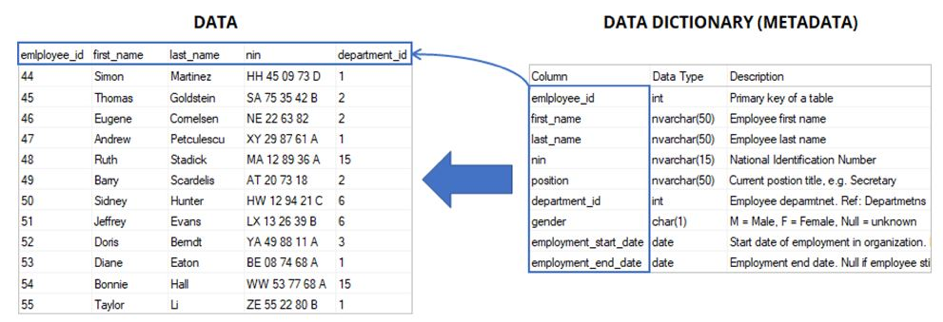
\includegraphics[width=.8\textwidth]{Content/images/modellierung/data.png}
    \caption{}
    \label{fig:modellierung:data}
\end{figure}

\subsection{Oracle Data-Dictionary}

Der Datenbankbenutzer SYS besitzt alle Basistabellen und vom Benutzer zugreifbaren Views des Data Dictionary.
Kein Oracle-Datenbankbenutzer sollte Zeilen oder Schemaobjekte im SYS-Schema ändern (UPDATE, DELETE oder INSERT), da diese Aktivitäten die Datenintegrität beeinträchtigen können.

Die Views des Data Dictionary dienen als Referenz für alle Datenbankbenutzer. Einige Ansichten sind für alle Oracle-Datenbankbenutzer zugänglich, andere nur für Datenbankadministratoren. 
Das Data Dictionary ist immer verfügbar und befindet sich im SYSTEM Tablespace.

Das Data Dictionary besteht aus Views. In vielen Fällen besteht eine Gruppe aus drei Views, die ähnliche Informationen enthalten und sich durch ihre Präfixe voneinander unterscheiden:

\begin{itemize}
    \item USER: Die Datenbankobjekte, die der Benutzer in seinem Schema angelegt hat
    \item ALL: Die Datenbankobjekte, auf die der Benutzer Zugriffsrechte erhalten hat 
    \item DBA: Alle angelegten Datenbankobjekte
\end{itemize}

Des Weiteren gibt es noch einen vierten Präfix (V\$), welcher für statistische Informationen, die für Laufzeitverbesserungen (Tuning) oder für optimierte Speicherformen ausgewertet werden können, verwendet wird.

Beispiele:
\textbf{Alle Objekte im eigenen Schema:}
\begin{lstlisting}
SELECT object\_name, object\_type FROM USER\_OBJECTS;    
\end{lstlisting}
\textbf{Alle Objekte auf die der Benutzer Zugriff hat:}
\begin{lstlisting}
SELECT owner, object\_name, object\_type FROM ALL\_OBJECTS;
\end{lstlisting}
\textbf{Globale Ansicht auf die Datenbank (wird vom Administrator ausgeführt):}
\begin{lstlisting}
SELECT owner, object\_name, object\_type FROM SYS.DBA\_OBJECTS;
\end{lstlisting}

\section{Sternschema (Star-Schema)}

Das Star-Schema ist, wie der Name schon beschreibt, sternförmig aufgebaut und für analytische Anwendungen im Data Warehouse-Umfeld geeignet.
Die Fakten (engl. Measures) in einem Star-Schema sind in diesem Modell das zentrale Element der Datenanalyse. Sie haben die Aufgabe wichtige Zusammenhänge in quantitativ messbarer und verdichteter Form wiederzugeben.
Die Dimensionen (engl. Dimensions) in einem Star-Schema ermöglichen unterschiedliche Sichten auf die Fakten. Sie liefern einen fachlichen Bezug auf die quantitativen Werte in einem Sternschema.

\begin{figure}[h]
    \centering
    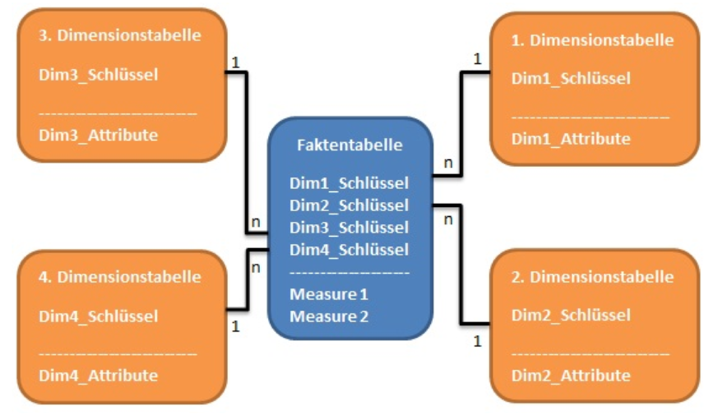
\includegraphics[width=.8\textwidth]{Content/images/modellierung/star.png}
    \caption{Aufbau}
    \label{fig:modellierung:star}
\end{figure}

Die Fakten können in einem Star-Schema gruppiert und analysiert werden. Die Betrachtung von Verdichtungsstufen ermöglicht die sogenannten Hierarchisierungen. Da im Star-Schema keine direkte Hierarchisierung von Dimensionen möglich ist, wird über die „kontrollierte Redundanz“ in den Dimensionen eine Hierarchisierung ermöglicht.
Das Star-Schema setzt sich aus Fakten- und Dimensionstabellen zusammen. Die Faktentabelle enthält einerseits die wichtigen Kennzahlen und andererseits speichert sie die Fremdschlüssel der Dimensionstabellen.

\paragraph{Vorteile}
\begin{itemize}
    \item einfaches, intuitives Datenmodell (Join-Tiefe nicht größer als 1)
    \item schnelle Anfrageverarbeitung
    \item Verständlichkeit und Nachvollziehbarkeit
\end{itemize}

\paragraph{Nachteile}
\begin{itemize}
    \item verschlechterte Antwortzeit bei häufigen Abfragen sehr großer Dimensionstabellen 
    \item Redundanz innerhalb einer Dimensionstabelle
    \item Aggregationsbildung ist schwierig
    
\end{itemize}

\paragraph{Ziel}
\begin{itemize}
    \item Benutzerfreundliche Abfrage 
\end{itemize}

\paragraph{Ergebnis}
\begin{itemize}
    \item Einfaches, lokales und standardisiertes Datenmodell
    \item Eine Faktentabelle und wenige Dimensionstabellen    
\end{itemize}

\begin{figure}[h]
    \centering
    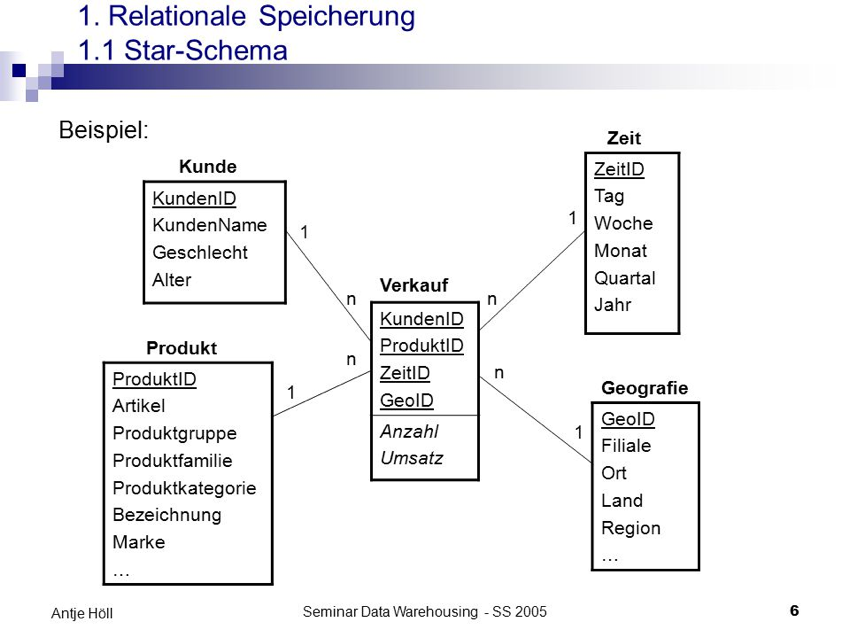
\includegraphics[width=.8\textwidth]{Content/images/modellierung/star2.png}
    \caption{Beispiel}
    \label{fig:modellierung:star2}
\end{figure}

\subsection{Schneeflockenschema (Snowflake-Schema)}

Das Snowflake-Schema ist eine weitere Variante Informationen in mehrdimensionalen Datenräumen zu speichern. Dabei ähnelt die Struktur des Datenmodells eines Datenmodells, das sich in der 3. Normalform befindet.
Das Snowflake-Schema (Schneeflockenschema) ist eine Weiterführung des Sternschemas. Im Snowflake-Schema wird jede weitere Hierarchiestufe durch eine weitere Datenbanktabelle realisiert.
Dadurch steigt die Anzahl von SQL Joins beim Schneeflockenschema im Gegensatz zum Sternschema linear mit der Anzahl der Aggregationspfade an.

\begin{figure}[h]
    \centering
    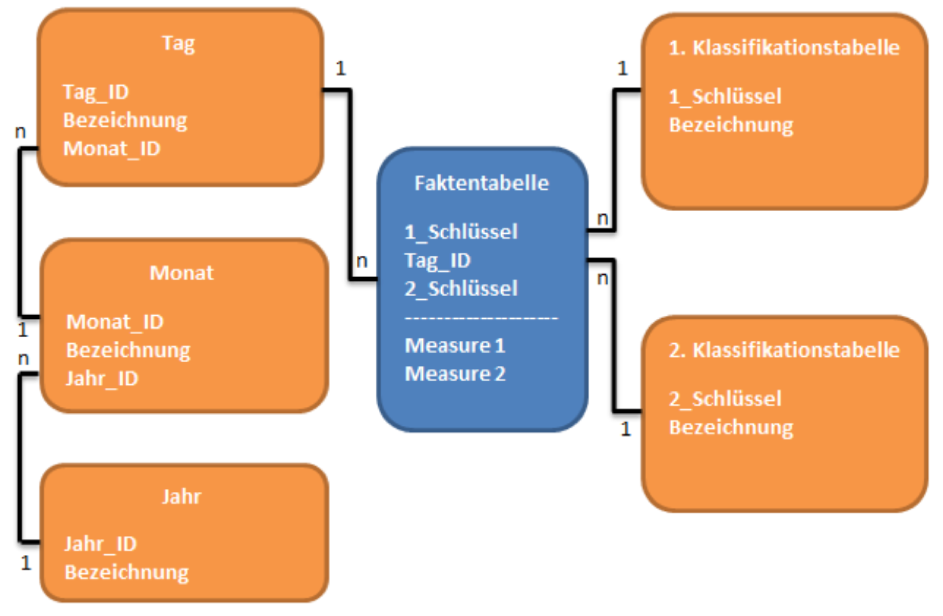
\includegraphics[width=.8\textwidth]{Content/images/modellierung/snow.png}
    \caption{Aufbau Snowflake Schema}
    \label{fig:modellierung:snow}
\end{figure}

Die Kennzahlen werden innerhalb einer Faktentabelle gespeichert. In der Faktentabelle sind numerische Fremdschlüsselbeziehungen zu den jeweils niedrigsten Hierarchiestufen der verschiedenen Dimensionen enthalten, gemäß der Granularität des Datenwürfels.
Jede weitere Hierarchiestufe wird in einer eigenen Tabelle angelegt und mittels 1:n Beziehungen an die vorherige Hierarchiestufe miteinander verbunden. Durch den Einsatz des Snowflake-Schemas entsteht ein sehr komplexes Datenmodell, welches die Ausprägung einer Schneeflocke hat.

\paragraph{Vorteile}
\begin{itemize}
    \item geringerer Speicherplatzverbrauch (keine redundanten Daten)
    \item n:m - Beziehungen zwischen Aggregationsstufen können über Relationstabellen aufgelöst werden
    \item optimale Unterstützung der Aggregationsbildung
    \item häufige Abfragen über sehr große Dimensionstabellen erbringen Zeitersparnis und Geschwindigkeitsvorteil (Browsing-Funktionalität)

\end{itemize}

\paragraph{Nachteile}
\begin{itemize}
    \item Komplexere Strukturierung: die Daten sind zwar weniger redundant, die Zusammenhänge sind jedoch komplexer als in einem Star-Schema
    \item größere Tabellenanzahl
    \item Reorganisationsproblem: Änderungen im semantischen Modell führen \newline zu umfangreicher Reorganisation der Tabellen und somit zu einem höheren Wartungsaufwand

\end{itemize}

\paragraph{Ziele}
\begin{itemize}
    \item Redundanzminimierung durch Normalisierung
    \item Effiziente Transaktionsverarbeitung

\end{itemize}

\paragraph{Ergebnis}
\begin{itemize}
    \item Komplexes und spezifisches Schema
    \item Viele Entitäten und Beziehungen bei großen Datenmodellen

\end{itemize}

\begin{figure}[h]
    \centering
    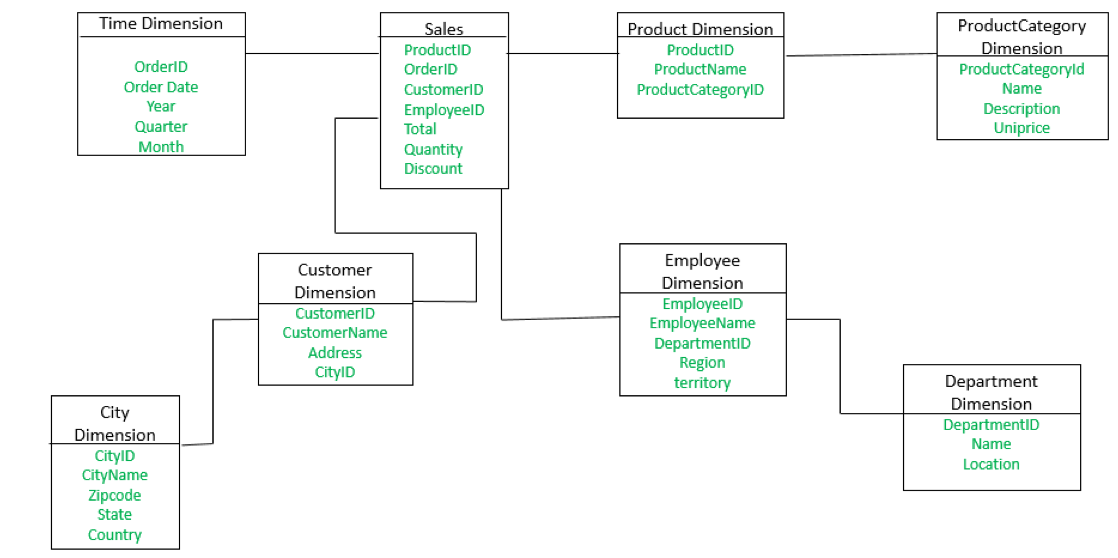
\includegraphics[width=.8\textwidth]{Content/images/modellierung/starb.png}
    \caption{Beispiel Snowflake}
    \label{fig:modellierung:starb}
\end{figure}

\section{Problem der Zeit}

Die Zeit kann man im relationalen Datenmodell nicht abbilden, außer man fügt zusätzliche Spalten ein. 

Es wird zwischen einer Zeitdauer mit Lücken und einer Zeitdauer ohne Lücken unterschieden. 

Beispiel: Tabelle mit Artikel und Preis

Der Kunde Max Meier kauft am 1. Februar 2020 einen Artikel. Drei Wochen später schickt er diesen zurück und möchte sein Geld zurückbekommen. Der Artikel kostet derzeit \euro{89}. Man kann jedoch nicht genau sagen, wie viel der Artikel am 1. Februar gekostet hat.

Lösung: In der Datenbank muss ein Feld sein, wo der Preis mit der Zeit eingetragen ist (\euro{89} bis 12.02.2020).

Bei einem zusätzlichen „bis“ Feld muss die Zeit ohne Lücken dargestellt werden. Eine Zeitdauer mit Lücken geht nur, wenn ein „von – bis“ Feld vorhanden ist.

Ähnlich ist es bei einer Materialverfolgung. Hier möchte man beispielsweise wissen, wann sich der Rohstoff X wo befindet. Deshalb muss die Zeit in Kombination mit dem Ort in einem Feld gespeichert werden. In Echtzeit kann das Material aber trotzdem nicht verfolgt werden, da mit dem zusätzlichen Zeit – Ort Feld lediglich feststellen kann, zwischen welchen Zeitpunkten sich das Material an welchem Ort befunden hat.
